\documentclass[12pt,a4paper]{article}

\usepackage[T1]{fontenc}
\usepackage[utf8]{inputenc}
\usepackage{times}
%\usepackage[sorting=none]{biblatex}

\newcommand{\mathDP}{\gamma^{\mathrm{D}}\ }
\newcommand{\mathmDP}{\mathrm{m}_{\mathDP}\ }
\newcommand{\DP}{$\mathDP$}
\newcommand{\mDP}{m$_{\mathDP}$}
\newcommand{\Br}{\mathop\mathrm{Br}}
\usepackage[usenames,dvipsnames,svgnames,x11names,table]{xcolor}
\usepackage{lineno}  % for line numbering during review
%Tables
\usepackage{tabularx}
%% Graphics
\usepackage{graphicx}  % to include figures (can also use other packages)
\usepackage{amsmath} % Adds a large collection of math symbols
\usepackage{amssymb}
\usepackage{amsfonts}
\usepackage{upgreek} % Adds in support for greek letters in roman typeset

\usepackage[font=footnotesize,labelfont=bf]{caption}
\usepackage[font=footnotesize,labelfont=bf]{subcaption}
\usepackage[colorlinks,linkcolor=Blue3]{hyperref}
\usepackage[all]{hypcap} % Internal hyperlinks to floats.


\begin{document}

\renewcommand{\thefootnote}{\fnsymbol{footnote}}
\setcounter{footnote}{1}

%------------------------------------
\title{Sensitivity of the SHiP experiment to Dark Photons}

\author{The SHiP collaboration}

\maketitle

\begin{abstract}

Dark photons are hypothetical new vector particles that could act as
mediators between our standard model particles and a hidden
sector. The simplest of such vector-portal models is fully
characterised by only two parameters: the mass of the dark photon
m$_{\gamma^{\mathrm{D}}}$ and its mixing parameter with the photon,
$\varepsilon$. The sensitivity of the SHiP detector is reviewed for
dark photons in the mass range between 0.01 and 10 GeV. Different
production mechanisms are simulated, with the dark photons decaying to
pairs of visible fermions. Exclusion contours are presented and
compared with those of other existing or planned experiments. The SHiP
detector is expected to have a unique sensitivity for
m$_{\gamma^{\mathrm{D}}}$ ranging between XX and XX GeV, and
$\varepsilon$ ranging between XX and XX.

\end{abstract}

\renewcommand{\thefootnote}{\arabic{footnote}}
\setcounter{footnote}{0}

\tableofcontents
\cleardoublepage

\pagestyle{plain} % restore page numbers for the main text
\setcounter{page}{1}
\pagenumbering{arabic}

\section{Introduction}
\label{sec:intro}

The CERN beam facility located near Geneva, Switzerland, comprises
several particle accelerators among which the Large Hadron Collider
(LHC)~\cite{LHC} is the World's largest and most energetic to
date. High-energy protons are delivered to the LHC by the Super Proton
Synchrotron (SPS). The 400-GeV proton beam of the SPS is also used in
fixed-target experiments. The LHC is planned to be upgraded into a
High-Luminosity machine around 2025 with the HL-LHC program
~\cite{Apollinari:2015bam}.

%The LHC has been delivering data at centre of mass energies of 7, 8
%and 13 TeV since 2010. The first milestone in its physics program was
%reached in 2012 with the discovery of the Higgs boson by the ATLAS and
%CMS collaborations~\cite{ATLAS,CMS}. Several other milestones remain,
%oriented towards searches for physics beyond the standard model
%involving new massive particles.

In parallel to the high-energy frontier probed by the LHC, another
complementary way of exploring the phase space to find new physics is
through the "intensity frontier". By probing lower-energy scenarios,
the aim is to identify whether the new physics could be hidden from
sight due to weak connections through portals instead of direct
interactions with the known particles, with the new particles living
in a hidden sector. The simplest extensions of the standard model (SM)
are possible through three types of portals, involving either a scalar
(e.g. dark Higgs boson), a vector (e.g. dark photon) or fermions
(e.g. heavy neutral leptons). Strong constraints exist already from
the LHC experiments on high-mass short-lived
mediators~\cite{Aaboud:2018fvk,Aaboud:2017buh,CMS-PAS-HIG-18-003,Khachatryan:2016zqb}. The
long-lived scenarios with relatively low masses remain however largely
unexplored. The SHiP (Search for Hidden Particles) experiment\cite{TP}
has been proposed in 2012 and designed to look for particles which
would decay in the range 50-120\,m from their production vertices. The
sensitivity of the SHiP detector to heavy neutral leptons has been
investigated in~\cite{SHiPPaper3}. This article is dedicated to
studying the sensitivity of the SHiP detector to dark photons.

After describing briefly the SHiP detector and its simulation in
section~\ref{sec:shipdetector}, the theory considered for the dark
photon production and decay is reviewed in
section~\ref{sec:DPprod}. The sensitivity of the SHiP detector is
given in section~\ref{sec:sensitivity} for the three production modes
studied and decay to visible fermions, in the minimal dark photon
model. Leptophilic and leptophobic scenarios are also
considered. Finally section~\ref{sec:concl} provides a conclusion.

\section{The SHiP Detector and Simulation}
\label{sec:shipdetector}

SHiP\cite{TP} is a new general purpose fixed target facility proposed
at the CERN SPS accelerator to search for particles predicted by
Hidden Portals.  These particles are expected to be predominantly
accessible through the decays of heavy hadrons. The facility is
therefore designed to maximise the production and detector acceptance
of charm and beauty mesons, while providing the cleanest possible
environment.  The 400 GeV proton beam extracted from the SPS will be
dumped on a high density target with the aim of accumulating $2\times
10^{20}$ protons on target (p.o.t.) during 5 years of operation.  The charm
production at SHiP exceeds any existing and planned facility.


A dedicated detector, based on a long vacuum tank followed by a
spectrometer and particle identification detectors, will allow probing
a variety of models with light long-lived exotic particles and masses
below $\mathcal O(10)~\rm{GeV/c^2}$.  Since the hidden sector
particles originating from charm and beauty are produced with a
significant transverse momentum with respect to the beam axis, the
detector should be placed as close as possible to the target.  A
critical component of SHiP is the muon shield, which deflects the high
flux of muons produced in the target, that would represent a very
serious background for the particle searches, away from the
detector. The detector is designed to fully reconstruct the exclusive
decays of hidden particles and to reject the background down to below
0.1 events in the sample of $2\times 10^{20}$ protons on target.  The
detector consists of a large magnetic spectrometer located downstream
of a 50 m-long and $5\times 10$ m-wide decay volume. To suppress the
background from neutrinos interacting in the fiducial volume, the
decay volume is maintained under a vacuum.  The spectrometer is
designed to accurately reconstruct the decay vertex, mass and impact
parameter
% ($\sigma_x=120\mu m$, $\sigma_{\rm{p}}/\rm{p}~\sim~0.5\%$) 
of the decaying particle at 
the target. A set of calorimeters 
%($\sigma_{\rm{E}}/\rm{E}~\sim~6\%/\sqrt{\rm{E}}$) 
followed by muon 
chambers provide identification of electrons, photons, muons and charged hadrons. 
A dedicated 
%high-resolution 
%(100 ps)
 timing detector measures the coincidence of the decay products, which
allows the rejection of combinatorial backgrounds.  The decay volume
is surrounded by background taggers to tag neutrino and muon inelastic
scattering in the surrounding structures, which may produce long-lived
SM $\rm{V}^0$ particles, such as $\rm{K}_{\rm{L}}$, that have similar
topologies to the expected signals.


The experimental facility is also ideally suited for studying
interactions of tau neutrinos.  It will therefore host an emulsion
cloud chamber based on the Opera concept, upstream of the
hidden-particle decay volume, followed by a muon spectrometer.


In the simulation, proton fixed target collisions are generated by
PYTHIA 8.2~\cite{Sjostrand:2014zea}, inelastic neutrino interactions by
GENIE~\cite{Genie} and inelastic muon interactions by
PYTHIA 6~\cite{pythia6}. The heavy flavour cascade production is also
taken into account~\cite{CERN-SHiP-NOTE-2015-009}.  The SHiP detector response is
simulated in the GEANT4~\cite{Geant4} framework. The simulation is
done within the FAIRROOT framework~\cite{FAIRROOT}.



\section{Dark photon production mechanisms}
\label{sec:DPprod}

The minimal dark photon model considers the addition of a \cal{U}(1)
gauge group to the SM, whose gauge boson is a vector field called the
dark photon \DP. A kinetic mixing between the dark
photon and the SM U(1) gauge bosons is allowed~\cite{Holdom:1985ag}, with a
reduced strength parametrised by a coupling $\varepsilon$, also called
the kinetic mixing parameter. In its simplest form, the knowledge of
the mass of the dark photon \mDP and the kinetic
mixing parameter $\varepsilon$ is enough to characterise the model and
calculate production cross section and decay properties.

Different mechanisms are possible for the production of such new
particles at a fixed-target experiment. Three different modes are
studied in this paper.

The initial 400 GeV proton beam interacts with the protons from the
target material, producing mesons. For meson decay channels involving
photons, there is a possibility for the photon to mix with the dark
photon, as described in subsection~\ref{sec:meson} below. This mode is
opened only for dark photon masses below 0.9 GeV, as for mesons with
masses above this threshold the main decay modes don't involve photons
anymore.

The proton-proton interaction could also lead to the radiation of a
dark photon via a bremsstrahlung process, as described in
subsection~\ref{sec:pbrem} below. This mode is heavily suppressed when
the dark photon mass is heavier than the Quantum Chromodynamic (QCD)
scale, so remains competitive only for masses below $\simeq 2$ GeV.

The last production mode studied here is via a Drell-Yan like QCD
process, or quark-quark annihilation into the dark photon, as
described in subsection~\ref{sec:qcd} below. For this to happen, the
dark photon mass can be in the 1-10 GeV range. Using the parton model
with a factorisation scale below the GeV scale cannot give sensible
results, as expected from the range of validity of parton distribution
functions, and hence this area of phase-space has not been considered
here.

In this paper, the assumption that only the initial proton interacts
is made. In reality, similar interactions could also happen from
protons coming from cascade decays happening in the target
material. For electromagnetic processes (electron bremsstrahlung of
photons mixing with the dark photon), it has been shown
in~\cite{Gorbunov:2014wqa} that their contribution is negligible
compared to the main production mechanisms described above. The study
however remains to be done for hadronic interactions in the cascade
decays, and will be the subject of future work. Hence the results
presented here are conservative and the sensitivity could be improved
in the future when this contribution is added.

The dark photon decay to pairs of visible fermions is considered as
described in subsection~\ref{sec:decay} below.


\subsection{Production in meson decay}
\label{sec:meson}

The Pythia 8.2~\cite{Sjostrand:2014zea} Monte Carlo (MC) generator is
used to produce inclusive QCD events in proton-proton collisions,
through all available non-diffractive processes. One proton beam
momentum is set to 400\,GeV and the other to 0 (protons from the fixed
target material). The total proton-proton cross section with a
corresponding center-of-mass energy of 27.43 GeV is predicted to be
$\sigma_{\mathrm{pp}}^{\mathrm{tot}} = 40.6 \pm
1.2$\,mb~\cite{Patrignani:2016xqp}, and the non-diffractive cross
section given by Pythia is $\sigma_{\mathrm{pp}}^{\mathrm{non-diff}} =
24$\,mb. The mesons that are produced are then used as sources of dark
photons, if they have decay modes to photons and their decay to a dark
photon of mass \mDP is kinematically allowed. Four processes are found
largely dominant (with other contributions neglected) and shown in
table~\ref{tab:mesonDecays}. The decay tables of these four mesons are
reset to having only one decay mode allowed with 100\% branching ratio
($\pi^{0}\rightarrow \gamma\gamma $,$\eta\rightarrow \gamma\gamma $,
$\omega\rightarrow \pi^{0}\gamma $, $\eta'\rightarrow \gamma\gamma
$). If several mesons of interest are produced, only the last one
encountered is considered.

The branching ratios of the mesons to these new decay modes are
function of the \mDP, the mixing parameter $\varepsilon$, the meson
type, pseudo-scalar or vector, and the meson
mass~\cite{Batell:2009di,Gorbunov:2014wqa}. For pseudo-scalar mesons
$\mathcal{P}$ ($\pi^0$, $\eta^0$ and $\eta^{\prime}$), the branching
ratio to \DP$\gamma$ is given by equation~\ref{eq:mesonBR1}. For
vector mesons $\mathcal{V}$ ($\omega$), the branching ratio to a \DP
and a pseudoscalar meson $\mathcal{P}$ is given by
equation~\ref{eq:mesonBR2}.

\begin{align}
	\Br(\mathcal{P}\to \mathDP \gamma)\simeq 2\epsilon^2\left ( 1-\frac{m_{\mathDP}^2}{m_{\mathcal{P}}^2} \right )^3 \Br(\mathcal{P}\to\gamma\gamma)\,,\label{eq:mesonBR1}
\end{align}

\begin{align}
\Br(\mathcal{V}^\pm\to \mathcal{P} \mathDP ) & \simeq \epsilon^2\times \Br(\mathcal{V}^\pm\to \mathcal{P} \gamma)\label{eq:mesonBR2} \\ 
&\times\frac{(m_{\mathcal{V}}^2-m_{\mathDP}^2-m_{\mathcal{P}}^2)^2\sqrt{(m_{\mathcal{V}}^2-m_{\mathDP}^2+m_{\mathcal{P}}^2)^2-4m_{\mathcal{V}}^2m_{\mathcal{P}}^2}}{(m_{\mathcal{V}}^2-m_{\mathDP}^2)^3}\,.\nonumber
\end{align}

For the branching ratios of the mesons to $\gamma\gamma$ or
$\gamma\pi^0$, the same values as implemented in Pythia 8.2 were
used. The average number of mesons produced per p.o.t.,
n$_{\mathrm{meson}}$ / p.o.t., is shown for each meson type in the
last column, from toy samples of 100,000 proton-on-target (p.o.t.)
non-diffractive collisions simulated with Pythia
8.230~\cite{Sjostrand:2014zea}. The uncertainty is set to the mean
deviation of the distributions obtained repeating the same simulations
1000 times.

%values from PDG don't add up to 1, so I understand from Pythia manual
%that they were ``adapted'' to sum-up to 1 somehow.... -> but maybe we
%would want to use PDG values here if we extract an uncertainty from
%this.

\begin{table}[thbp]
  \centering
  \begin{tabular}{|l|c|c|c|}
\hline
\mDP (GeV) & meson &  BR($\gamma+X$)~\cite{Sjostrand:2014zea} & n$_{\mathrm{meson}}$ / p.o.t. \\
\hline 
0-0.135  &    $\pi^{0}\rightarrow\mathDP\gamma$ &  0.98799 &  $6.147 \pm 0.003$ \\
0.135-0.548  &   $\eta\rightarrow\mathDP\gamma$ &  0.3931181 &  $0.703 \pm 0.008$\\
0.548-0.648  &   $\omega\rightarrow\mathDP\pi^0$ & 0.0834941 &  $0.825 \pm 0.009$ \\
0.648-0.958  &    $\eta'\rightarrow\mathDP\gamma$ & 0.0219297 & $0.079 \pm 0.003$ \\
\hline
\end{tabular}
  \caption{Meson decay modes considered for the \DP production.}
  \label{tab:mesonDecays}
\end{table}


The cross section for the production of dark photon via meson decays
produced in non-diffractive primary interactions of the proton beam is
then computed as in equation~\ref{eq:mesonRate}, using
equations~\ref{eq:mesonBR1} and~\ref{eq:mesonBR2} and values reported
in table~\ref{tab:mesonDecays}. The cross section is proportional to
$\varepsilon^2$.

\begin{align}
	\sigma_{\mathrm{meson}} = \frac{\sigma_{\mathrm{pp}}^{\mathrm{non-diff}}}{\sigma_{\mathrm{pp}}^{\mathrm{tot}}} \times n_{\mathrm{meson}} \mathrm{/ p.o.t.} \times \Br(\mathrm{meson}\to \mathDP+X)\,.\label{eq:mesonRate}
\end{align}

\textcolor{red}{@TODO: Add this factor
  $\frac{\sigma_{\mathrm{pp}}^{\mathrm{non-diff}}}{\sigma_{\mathrm{pp}}^{\mathrm{tot}}}
  = 24/40 = 0.6$ to the limit calculations. I don't think it is
  reasonable to assume what we are missing from cascade interactions
  will compensate for this: for now we have no idea of the spectrum in
  angle / momentum coming out of cascade decays....}

\subsection{Production in proton bremsstrahlung}
\label{sec:pbrem}

In analogy with ordinary photon bremsstrahlung of scattering protons,
the same process is used for dark photon production by scattering of
the incoming 400 GeV proton beam on the target protons. Following
references~\cite{Blumlein:2013cua, Gorbunov:2014wqa}, the differential
\DP production cross section can be expressed as in
equation~\ref{eq:pbremXS}:

\begin{align}
	\frac{d N}{dz dp_\perp^2} &= \frac{\sigma_{pp}(s')}{\sigma_{pp}(s)}\,
	w_{ba}(z,p_\perp^2)\,,\label{eq:pbremXS}\\
w_{ba}(z,p_\perp^2) &= \frac{\epsilon^2 \alpha_{QED}}{2\pi H}
\left[\frac{1+(1-z)^2}{z} -2z(1-z)\left(\frac{2m_p^2+m_{\mathDP}^2}{H}
-z^2\frac{2m_p^4}{H^2}\right) \right. \nonumber \\
&\left.+2z(1-z)\big(1+(1-z)^2\big)\frac{m_p^2m_{\mathDP}^2}{H^2}
+2z(1-z)^2\frac{m_{\mathDP}^4}{H^2} \right]\,.\nonumber
\end{align}

where $\sigma_{pp}(s/s')$ are the inelastic proton-proton
cross-sections evaluated for the incoming/outgoing proton energy
scales, $m_p$, $P$ and $E_p$ are the proton beam mass (set to $m_p =
0.938272081$\,GeV/c~\cite{Patrignani:2016xqp}) and initial momentum
and energy respectively, $p$ and $E_{\mathDP}$ are the momentum and
energy of the generated dark photon respectively, $p_\perp$ and
$p_\parallel$ are the components of the \DP momentum orthogonal and
parallel to the direction of the incoming proton respectively,
$\alpha_{QED}$ is the fine structure constant of Quantum
Electro Dynamic (QED), set to 1/137, $s'=2m_p(E_p-E_{\mathDP})$,
$s=2m_pE_p$ and
$H(p^2_\perp,z)=p_\perp^2+(1-z)m_{\mathDP}^2+z^2m_p^2$.

However, the above formula does not take into account possible QCD
contributions when the energy scale $Q^2$ of the process exceeds the
QCD scale, and the bremsstrahlung process starts to depend on the
internal partons. When the mass of the dark photon is much in excess
of 1~GeV, the standard dipole form
factor~\cite{RevModPhys.35.335} is included in the proton-\DP vertex,
leading to a penalty factor that models the strong suppression of the
bremsstrahlung production:

\begin{align}
	\mathrm{penalty}(m_{\mathDP}) = {\left(\frac{m_{\mathDP}^2}{0.71\,\mathrm{GeV}^2}\right)}^{-4}\quad \mathrm{ for }\quad m_{\mathDP}^2 > 0.71\,\mathrm{GeV}^2,
\end{align}

According to reference~\cite{Gorbunov:2014wqa}, this form factor is
conservative and probably underestimates the rates. As we are however
considering direct parton-parton QCD production in
section~\ref{sec:qcd}, to avoid double-counting this conservative
option is adopted.

The inelastic proton-proton cross-section $\sigma_{pp}(s)$ is taken
from experimental data:
\begin{align}
\sigma_{pp}(s) = Z + B\cdot \log^2\left(\frac{s}{s_0}\right) + Y_1\left(\frac{s_1}{s}\right)^{\eta_1} - 
Y_2\left(\frac{s_1}{s}\right)^{\eta_2},
\end{align}
where $Z = 35.45$~mb, $B = 0.308$~mb, $Y_1 = 42.53$~mb, $Y_2 = 33.34$~mb, $\sqrt{s_0} = 5.38$~GeV, 
$\sqrt{s_1} = 1$~GeV, $\eta_1 = 0.458$ and $\eta_2 = 0.545$~\cite{Agashe:2014kda}.

Reformulating equation~\ref{eq:pbremXS} as a function of the \DP angle
$\theta$ to the beam line and its total momentum p, a two-dimensional
normalised probability density function (PDF) $f(p, \theta)$ is
extracted, and shown in figure~\ref{fig:pbremPDF} for two choices of
\mDP. Note that due to the simple dependency of the production rate
scaling as $\varepsilon^2$, the normalised PDF is independent of
$\varepsilon$. The dark photons are generated with maximum probability
on each side of the beam axis ($\theta$ close to 0) with a factor of 5
more chance to have p$<100$ GeV compared to p$>200$\,GeV, for the low
masses, and increased probability to have high momentum as the mass
increases, with the highest probability to have the maximum momentum
available for \mDP$=2$\,GeV.

\textcolor{red}{@TODO: Investigate divergence at high masses - high momentum: seems unphysical.}

\begin{figure}[h!]
  \centering
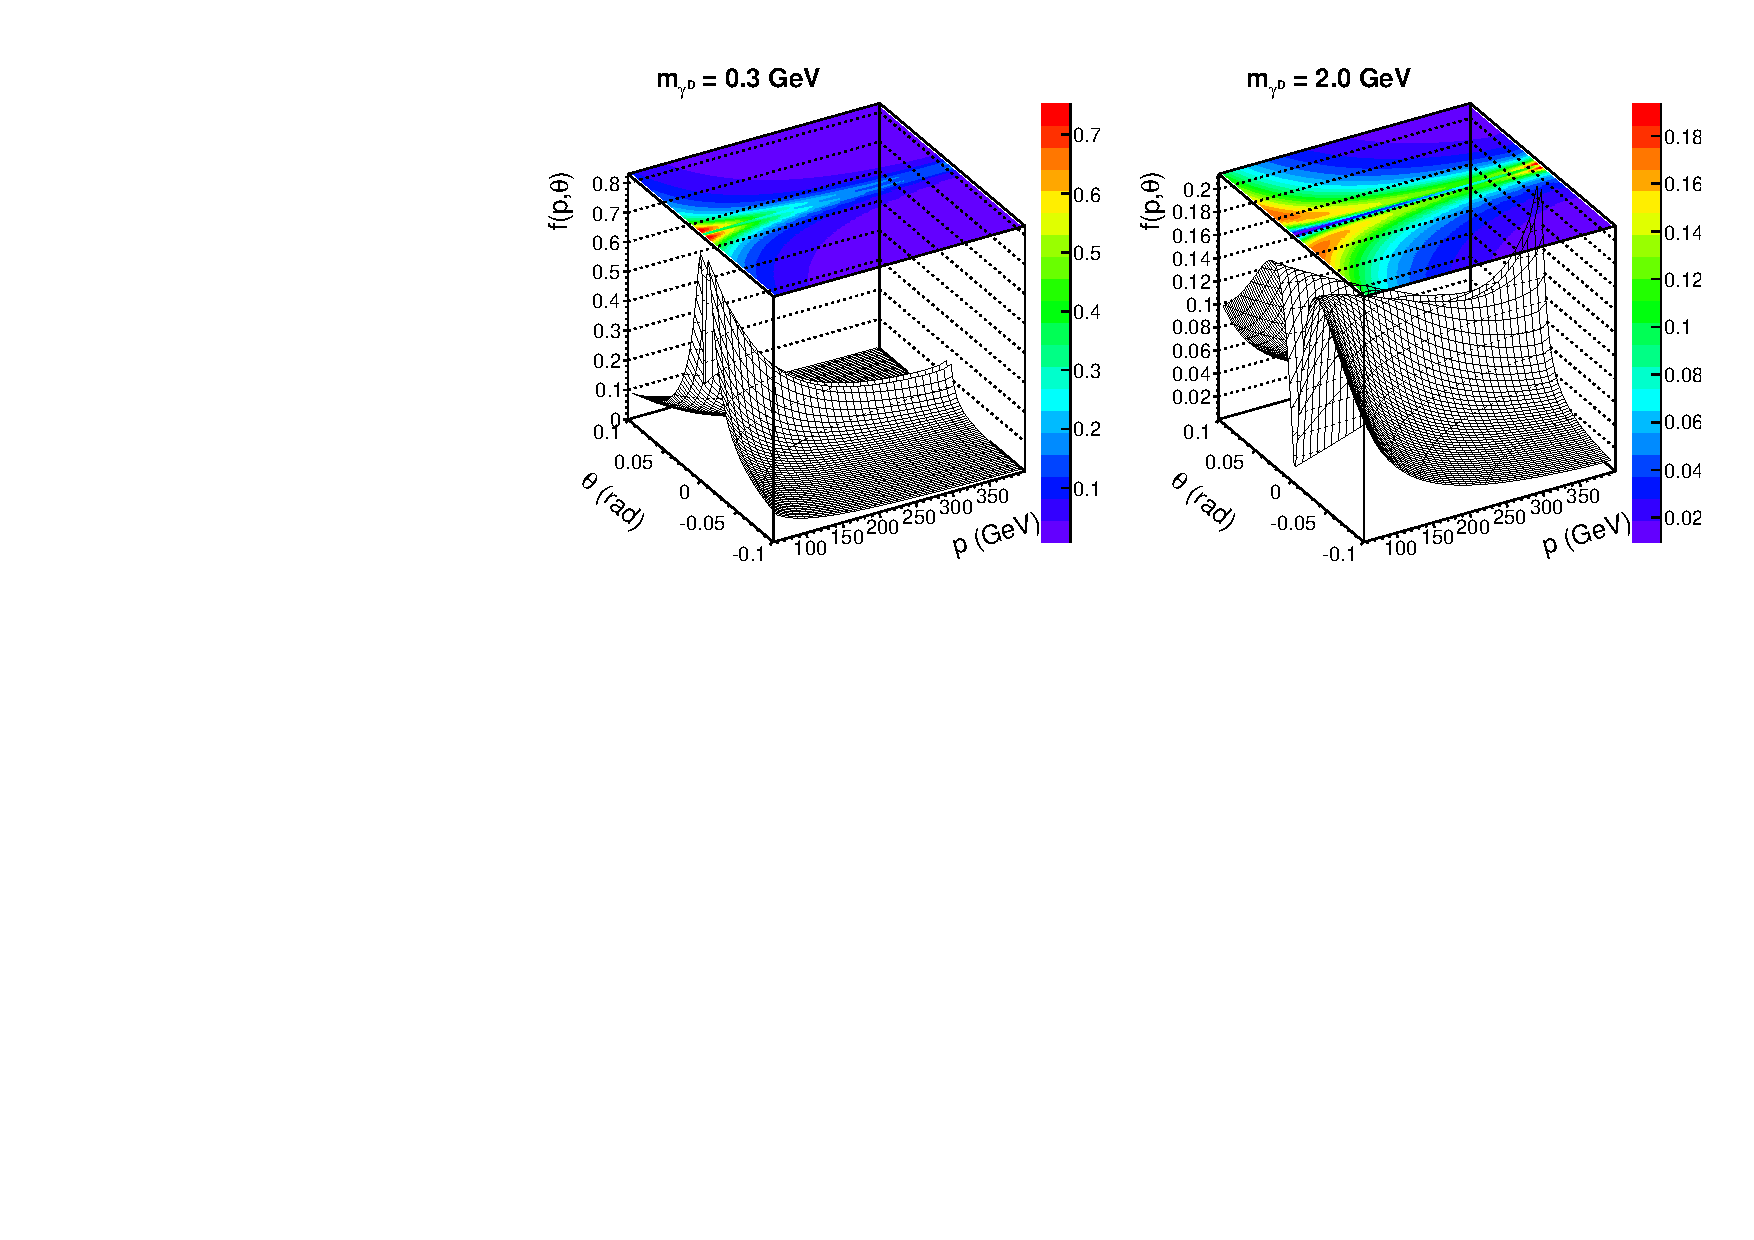
\includegraphics[width=1.\textwidth]{figures/pbrem_PDF.pdf}
\caption{Normalised probability density function of producing a dark
  photon with angle $\theta$ and momentum p through proton
  bremsstrahlung, for two examples of \mDP: 0.3\,GeV (left) and
  2\,GeV (right).}
\label{fig:pbremPDF}
\end{figure}


Events are generated using the Pythia8 gun with the \DP as particle,
randomly choosing the \DP(p, $\theta$) values according to the
normalised 2D PDF $f(p, \theta)$, extracted for each \mDP point
studied.

The integral of $f\times\mathrm{penalty}(m_{\mathDP})$ in the
kinematically allowed range of momenta, and complete solid angle
$\theta$($-\pi/2,\pi/2$), provides an estimate of the total dark
photon production rate $\sigma_{\mathrm{pbrem}}$ through proton
bremsstrahlung, scaling as $\varepsilon^2$. The conditions of validity
of the approximation used to derive
equation~\ref{eq:pbremXS}~\cite{KIM1972665, Kim_Tsai_1973} require a
lower momentum bound for the \DP at $p_{min}=0.14
P_p$~\cite{Blumlein:2013cua}, the upper bound being given by the
incoming 400\,GeV proton beam and \mDP.


\subsection{Drell-Yan production}
\label{sec:qcd}

For production of the dark photon in parton-parton scattering, the
generic implementation of a resonance that couples both to SM fermion
pairs and hidden particles is used, as implemented in Pythia 8.2 under
the ``HiddenValley'' Z' model~\cite{Carloni:2011kk}. A cross-check
has been done that similar kinematic distributions for the dark
photons are found using another Z' implementation in Pythia from
the ``New Gauge Bosons'' class of processes~\cite{Ciobanu:2005pv}.

The dark photons are generated in the mass range $1 < \mathmDP <
10$\,GeV. Below 1\,GeV one leaves the domain of perturbative QCD and
the parton model cannot be used anymore.

The cross section given by Pythia when the new particle has the
properties of the dark photon is shown in figure~\ref{fig:qcdXS}. Like
for the meson and proton bremsstrahlung processes, it is found to
scale as $\varepsilon^2$. An empirical function is extracted to
parametrise the cross section as a function of the \DP mass in a
continuous way, described in equation~\ref{eq:qcdXS}.

\begin{align}
  1 < \mathmDP \leq 1.4\,\mathrm{GeV} & : \sigma_{\mathrm{QCD}} =  0.0586-0.09037\times \mathmDP + 0.0360743\times \mathmDP^2\,, \label{eq:qcdXS} \\
  1.4 < \mathmDP \leq 3\,\mathrm{GeV} & : \sigma_{\mathrm{QCD}} =  e^{-3.802-1.532\times \mathmDP}\,, \nonumber \\
  \mathmDP > 3\,\mathrm{GeV} & : \sigma_{\mathrm{QCD}} =  e^{-5.673-0.8869\times \mathmDP}. \nonumber
\end{align}


\begin{figure}[h!]
  \centering
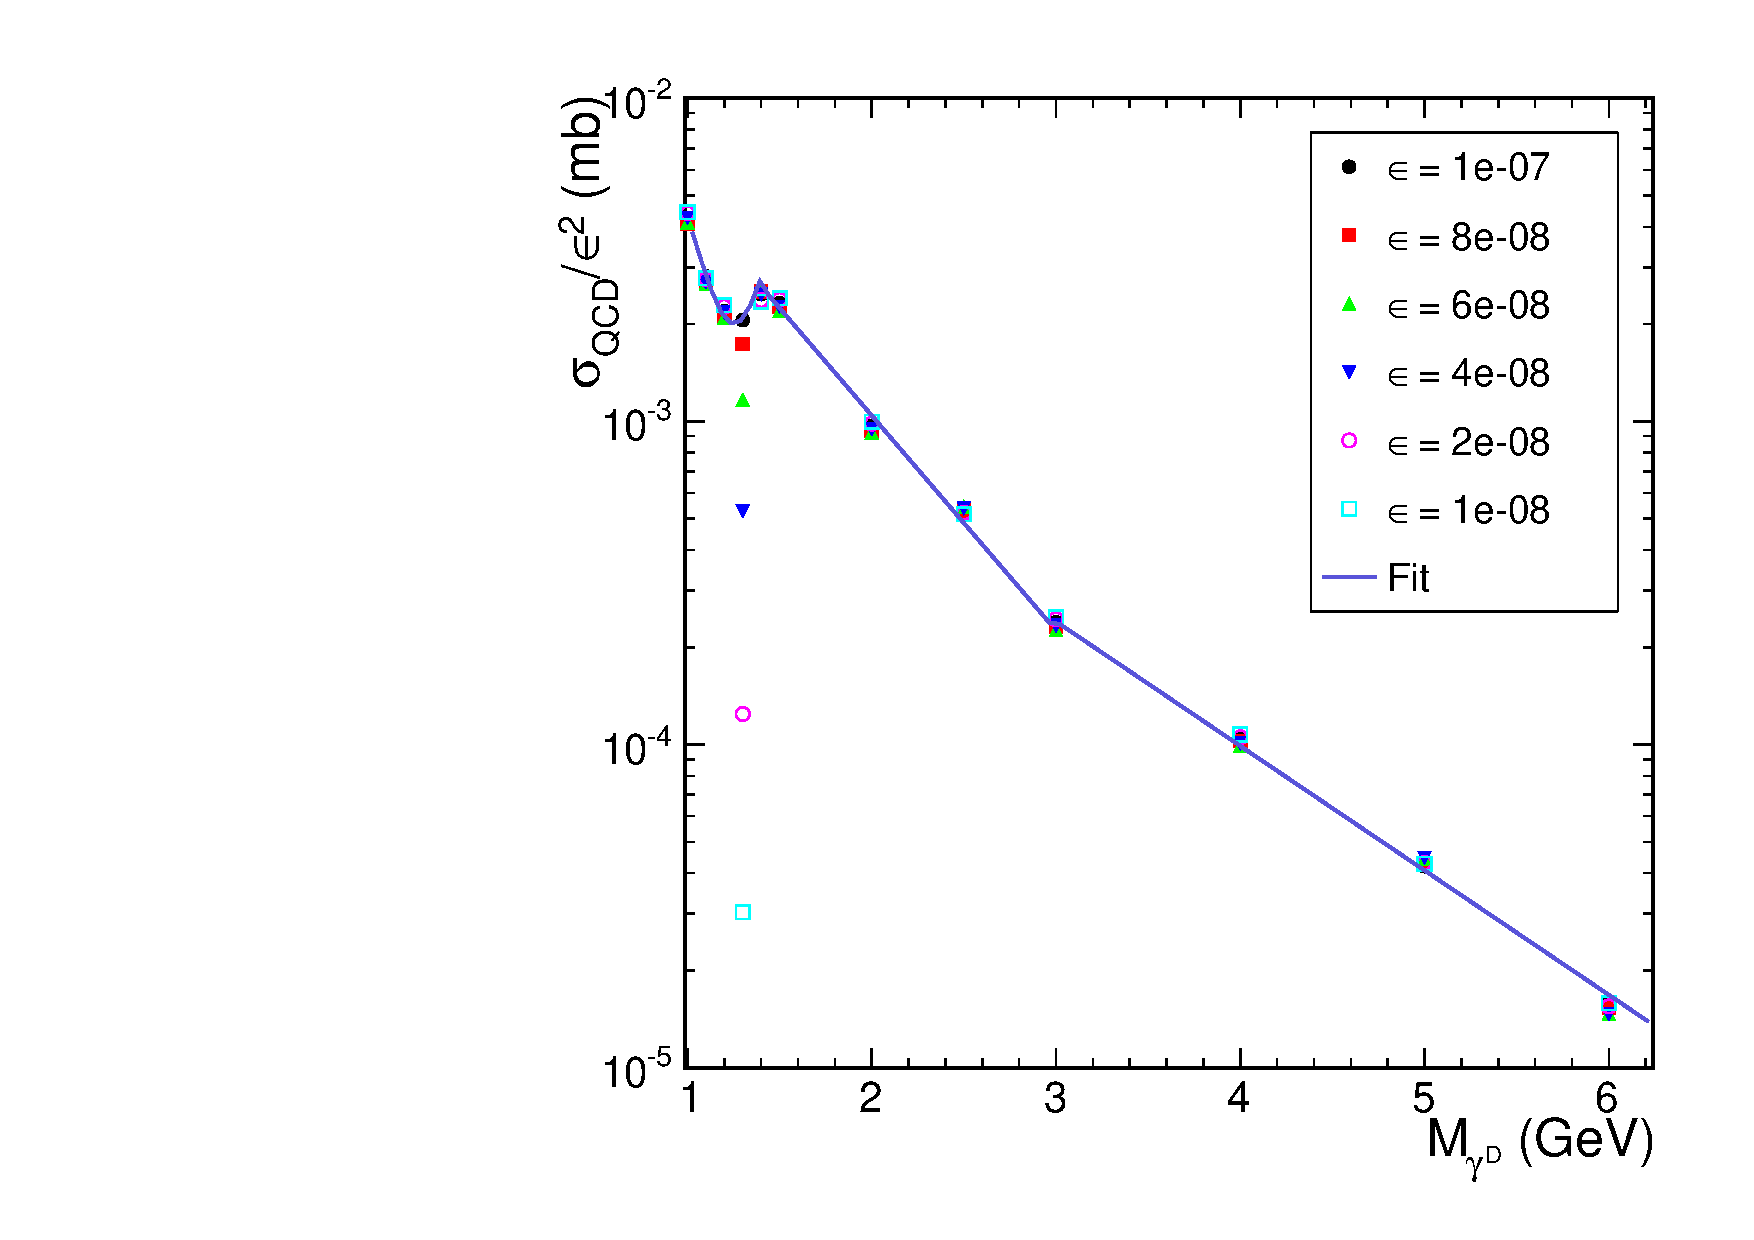
\includegraphics[width=1.\textwidth]{figures/qcdXSnorm_massFit.pdf}
\caption{QCD production cross section as a function of \mDP, for
  different values of $\varepsilon$. The fit function is described in
  equation~\ref{eq:qcdXS}.}
\label{fig:qcdXS}
\end{figure}

\textcolor{red}{@TODO: Drop anything below 1.4 GeV ? Discontinuity seems weird... Probably PDF evolution is already not good, 1.4 GeV was quoted by Steven Mrenna (Pythia8)....}

\textcolor{red}{@TODO: Add figure of the relative contributions from each process as a function of \mDP.}


\subsection{Dark photon decays}
\label{sec:decay}

Except for the meson production mode, in which the new particle
couples to the parent meson via mixing with the photon and hence
cannot be a resonance from Pythia's point-of-view, in QCD and proton
bremsstrahlung the \DP is made a proper resonance. In all cases, the
decay modes are implemented by hand as follows.

The partial decay width of the dark photon into a lepton pair is given by~\cite{Blumlein:2013cua}:
\begin{align}
	\Gamma(\mathDP \rightarrow l^+ l^-) = \frac{1}{3} \alpha_{\rm QED} m_{\mathDP} \epsilon^2 \sqrt{1 - \frac{4 m_l^2}{m_{\mathDP}^2}}\left(1 + \frac{2 m_l^2}{m_{\mathDP}^2}\right)~,\label{eq:dp-decay}
\end{align}
where $m_l$ is the lepton mass, for electron, muon or tau leptons, if
kinematically allowed. Following the approach used by the authors
of~\cite{Bjorken:2009mm}, the partial decay width into quark pairs is
computed as:
\begin{align}
	\Gamma(\mathDP \rightarrow~\text{hadrons}) = \frac{1}{3} \alpha_{\rm QED} m_{\mathDP} \epsilon^2 
	R\left(m_{\mathDP}\right)~,
\end{align}
where
\begin{align}
	R\left(\sqrt{s}\right) = \frac{\sigma(e^+e^- \rightarrow hadrons)}{\sigma(e^+e^- \rightarrow \mu^+\mu^-)}
\end{align}
is the energy-dependent R-ratio quantifying the hadronic annihilation
in $e^+e^-$ collisions~\cite{Agashe:2014kda}, tabulated from 0.3 to
10.29 GeV.


The lifetime of the \DP is then naturally set to the inverse of its
total width, summing all the kinematically-allowed channels in
calculating the total width. It is proportional to
1/$\varepsilon^2$. The branching ratios to individual channels are set
to the ratio of the partial over total width, and are hence
independent of $\varepsilon$. For separating the hadronic channels
into the different quark-flavoured pairs, the same relative branching
ratios as those of the SM Z bosons are used, namely: 0.22031,
0.17089, 0.22029, 0.17066, 0.21785 for decays to
$\mathrm{u}\bar{\mathrm{u}}$, $\mathrm{d}\bar{\mathrm{d}}$, $\mathrm{s}\bar{\mathrm{s}}$,
$\mathrm{c}\bar{\mathrm{c}}$, $\mathrm{b}\bar{\mathrm{b}}$,
respectively~\cite{Sjostrand:2014zea}. When the \DP is a resonance,
the decay goes explicitly through the pair of quarks, before
hadronisation. However in the case of the meson production, the
hadrons are found as direct decay products of the \DP.

The branching ratio of the \DP into the different final states is
shown in figure~\ref{fig:decayBR} as a function of \mDP. The hadronic
decays become available above the pion mass threshold. The expected
lifetime of the \DP as a function of its mass and $\varepsilon$ mixing
parameter is shown in figure~\ref{fig:ctau}.


\begin{figure}[h!]
  \centering
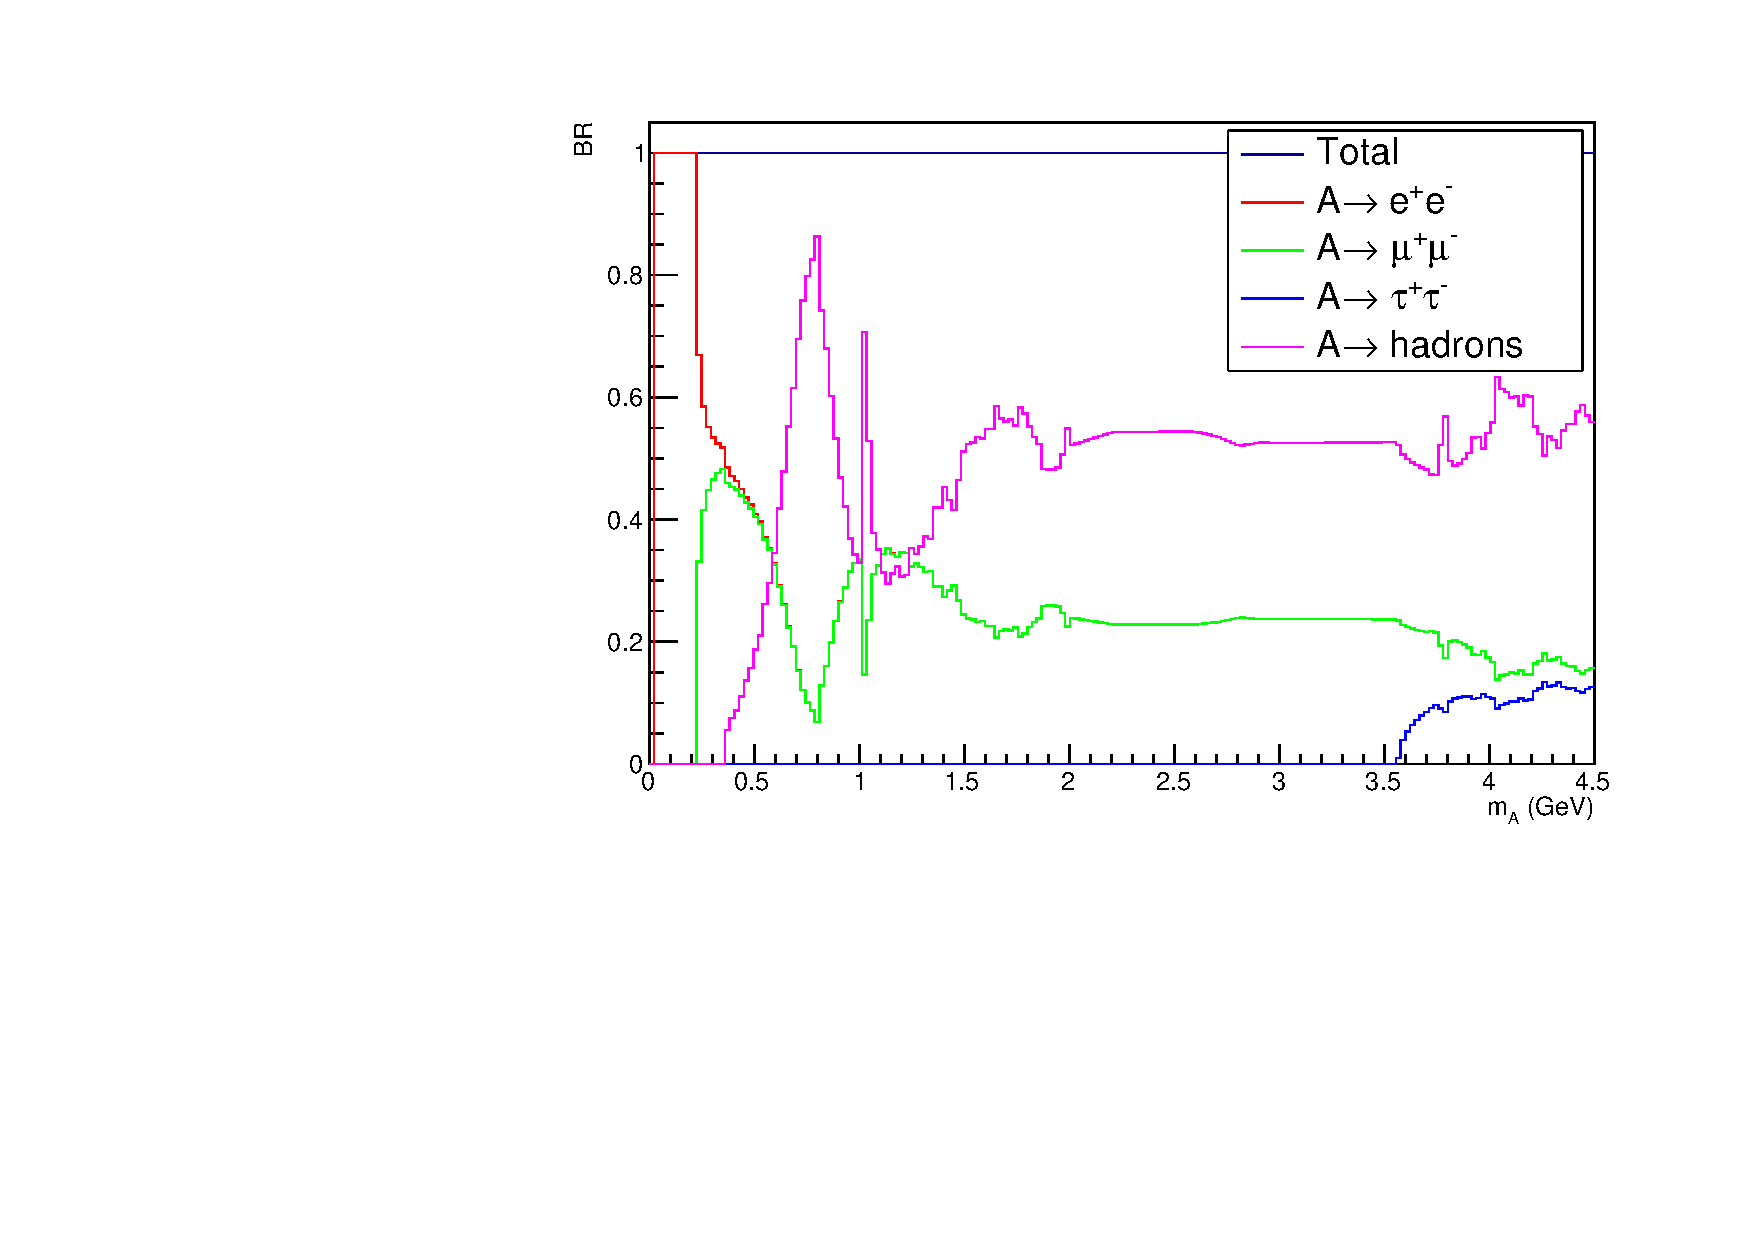
\includegraphics[width=1.\textwidth]{figures/BRvsmass.pdf}
\caption{Branching ratio of the \DP into fermion pairs as a function
  of its mass.}
\label{fig:decayBR}
\end{figure}


\begin{figure}[h!]
  \centering
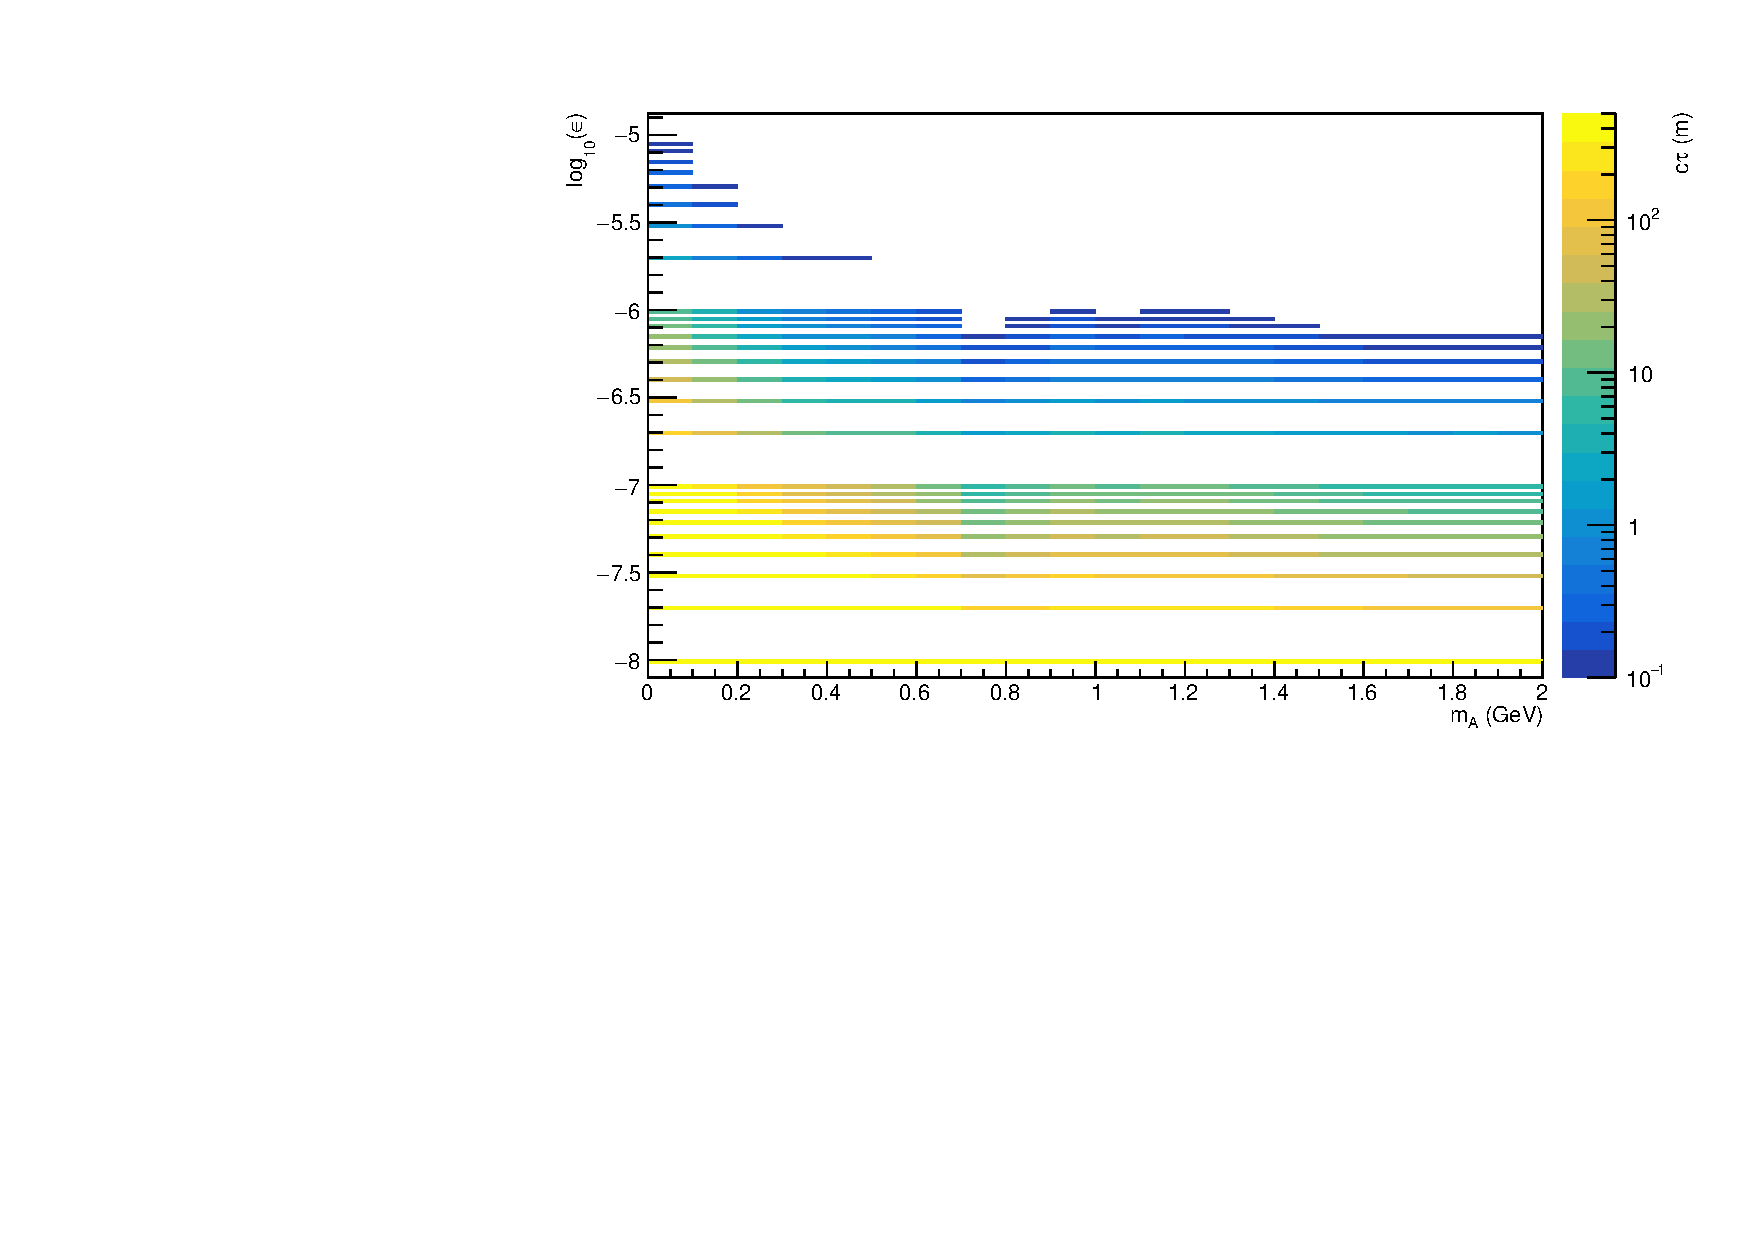
\includegraphics[width=1.\textwidth]{figures/ctauvsmassvseps.pdf}
\caption{Expected lifetime of the dark photon as a function of its mass and of the kinetic mixing parameter $\varepsilon$.}
\label{fig:ctau}
\end{figure}



\section{SHiP sensitivity}
\label{sec:sensitivity}

In order to maximise the usability of the events produced by Pythia in
the different production modes, the \DP decay vertex position is
randomly assigned to be inside the decay vessel of length
L$_{\mathrm{Vessel}}= 50.760$\,m, and the associated probability of
this happening is given as a function of the \DP quadrivector (p,
E$_{\mathDP}$) and lifetime $\mathrm{c}\tau$ by
equation~\ref{eq:decayVtx}.

\begin{align}
\mathrm{w}_{\mathrm{vtx}}(\ell) = e^{\frac{-\ell}{\beta\times\gamma\times \mathrm{c}\tau}}\times \frac{\mathrm{L}_{\mathrm{Vessel}}}{\beta\times \gamma \times \mathrm{c}\tau}\,,\label{eq:decayVtx}
\end{align}

with $\gamma = E_{\mathDP}/\sqrt{E_{\mathDP}^2-p^2}$, $\beta =
p/E_{\mathDP}$ and $\ell$ randomly distributed between 0 and
L$_{\mathrm{Vessel}}$ with a flat prior.

The total event rate expected is then expressed in
equation~\ref{eq:totalRate}, for each production mode $\mathrm{m}$
(meson, proton bremsstrahlung, QCD):

\begin{align}
	n(\mathDP | \mathrm{m}) = \mathrm{N\,(p.o.t.)} \times \sigma_{\mathrm{m}}(pp \to \mathDP) \times  \int_{\mathrm{Vessel}} \mathrm{w}_{\mathrm{vtx}}(\ell)\mathrm{d}\ell  \times \mathcal{A}_{\mathrm{det}}\,,\label{eq:totalRate}
\end{align}

$\mathrm{N\,(p.o.t.)} = 2 \times 10^{20}$ is the total number of
p.o.t. expected by the end of the SHiP physics program, and
$\mathcal{A}_{\mathrm{det}}$ is the detector acceptance times efficiency
to reconstruct the decay products in the SHiP detector and is
described in detail in section~\ref{sec:reco}.

The strategy of the analysis relies on identifying the decays of the
\DP into at least two charged particles. The reconstructed charged
tracks must originate from a common vertex. These requirements are
enough to ensure that no background event will survive the selection,
as demonstrated in~\cite{TP,PP}.  The 90\% confidence level (CL) limits on
the existence of a \DP with given (\mDP, $\varepsilon$) are hence set
by excluding regions where more than 2.3 events are expected.

\subsection{Decay modes}

The following decay modes are considered, whenever available according
to \mDP: e$^{+}$e$^{-}$, $\mu^{+}\mu^{-}$, $\pi^{+}\pi^{-}+X$,
K$^{+}$K$^{-}$, $\tau^{+}\tau^{-}$ in one-prong decay modes, and any
other hadronic decay modes leading to two charged particles passing the
selection from section~\ref{sec:reco}.

\textcolor{red}{@TODO: Add one plot (BR independent of production
  mode...), showing full mass range 0.1 to 6 GeV, possibly in log
  scale for the mass axis is better visibility of the decay modes,
  with the final state particles BR vs mass, for these categories:
  e+e- and mu+mu- together, tau+tau- in 1-prong decays,
  $\pi^{+}\pi^{-}+X$, K$^{+}$K$^{-}$, and all the others as
  ``others'', and their sum (the difference between that sum and 1
  being the decay modes we are not accessible to due to two charged
  tracks selection).}

\subsection{Vessel acceptance}

\textcolor{red}{@TODO: Plot of the vessel acceptance as a function of
  \DP mass, for decay modes like above, and separately
  for meson, pbrem, qcd. Also do couple of epsilon values ?}

\subsection{Reconstruction of the decay products}
\label{sec:reco}

The strategy employed in this analysis relies uniquely on the
reconstruction of charged particles by the SHiP straw tracker. Future
extensions of this work could consider also calorimeter deposits (to
tag e.g. photons from $\pi^0$ decays) and muon detectors. Events are
retained if two tracks are found passing the criteria summarised in
table~\ref{tab:recoSel}, namely that the two tracks are within the
fiducial area of the detector up to the fourth layer after the magnet,
the fit converged with good quality requirements, they have impact
parameters less than 0.1\,m in the (x,y) plane and a momentum above
1\,GeV. Criteria on the number of hits (NDF$>25$) or presence of hits
before/after the magnet are meant to reduce backgrounds which could
come from particles re-entering the detector volume due to the
magnetic field.

\begin{table}[thbp]
  \centering
  \begin{tabular}{|p{0.5\textwidth}|p{0.5\textwidth}|}
    \hline
    Decay vertex & z between straw veto tagger and exit lid of vacuum vessel \\
    & x-y within vessel volume \\
    \hline
    Straw tracker hits & in each layer - before and after magnet - up to station 4 \\
    \hline
    Tracks & NDF $> 25$, $\chi^2 / NDF < 5$, doca $<1$\,cm \\
    & >=2 tracks \\
    & p$>1$ GeV, IP$<0.1$\,m \\
\hline
\end{tabular}
  \caption{Selection criteria applied on the reconstructed events.}
  \label{tab:recoSel}
\end{table}



\textcolor{red}{@TODO: Describe selection requirements better, those driven
  by detector fiducial and fit quality, and those applied to reduce
  backgrounds. Plot reco efficiency for different decay modes like above,
  ee+mumu, tautau, hadrons, and separately for meson, pbrem, qcd, vs
  DP mass.}


\subsection{Systematic uncertainties}

The following sources of systematic uncertainties from theory are
investigated, for the three modes. They concern only the overall
normalisation, and not the impact from modifying the shapes of the \DP
kinematic variables, for which we rely on Pythia 8 (for meson and QCD
production) or available theoretical assumptions for the proton
bremsstrahlung production as described in section~\ref{sec:pbrem}.

For the meson production, the overall rate is affected by the
following uncertainties:
\begin{itemize}
\item which meson is chosen to give the kinematical properties of the
  event: first, last (central choice up to now), random. Because only
  one meson channel per mass range is considered, the impact is small:
  \textcolor{red}{@TODO: evaluate impact}
\item Branching ratios from table~\ref{tab:mesonDecays}:
  from~\cite{Patrignani:2016xqp}, the uncertainties on the measurement
  of these branching ratios are 0.03\%, 0.5\%, 3.4\% and 3.6\% for
  $\pi^0\rightarrow\gamma\gamma$, $\eta^0\rightarrow \gamma\gamma$,
  $\omega\rightarrow \pi^{0}\gamma$ and $\eta^{\prime}\rightarrow
  \gamma\gamma$ respectively, translating directly to the final rate.
\item uncertainty on n$_{\mathrm{meson}}$ / p.o.t.: from Pythia 8, as
  detailed in section~\ref{sec:meson} and table~\ref{tab:mesonDecays},
  they amount to 0.05\%, 1.1\%, 1.1\% and 3.8\% for $\pi^0$, $\eta^0$,
  $\omega$ and $\eta^{\prime}$ respectively, also translating directly
  to the final rate.
\item uncertainty on
  $\frac{\sigma_{\mathrm{pp}}^{\mathrm{non-diff}}}{\sigma_{\mathrm{pp}}^{\mathrm{tot}}}$:
  the uncertainty on $\sigma_{\mathrm{pp}}^{\mathrm{tot}}$ is
  3\%. \textcolor{red}{@TODO: evaluate impact for Pythia sigma
    non-diff, I don't know QCD uncertainties on this, presumably
    standard QCD scales and PDF uncertainties to be evaluated... It
    will probably end up dominant ?? }
\item theory uncertainties on branching ratio of mesons to dark
  photons: \textcolor{red}{??}
\item Missing contributions from cascade decays (future work).
\end{itemize}

For the proton bremsstrahlung, the theory systematic uncertainties concern:
\begin{itemize}
\item uncertainties on the inelastic proton-proton cross-section
  $\sigma_{pp}(s)$ will mostly cancel in the ratio
  $\frac{\sigma_{pp}(s')}{\sigma_{pp}(s)}$ so are neglected.
\item dipole form-factor: could consider no form-factor, but stopping
  bremsstrahlung production exactly where QCD production starts, at
  1.4\,GeV, and take difference as systematic.
\item uncertainty on w$_{ba}$: \textcolor{red}{??}
\item divergence at high p for high masses : \textcolor{red}{to be investigated}.
\item lower bound on p: \textcolor{red}{?}
\item Missing contributions from cascade decays (future work).
\end{itemize}

For the QCD production, the theory systematic uncertainties concern:
\begin{itemize}
\item Parametrisation of the cross section, impact from QCD scales and
  PDFs: \textcolor{red}{to be evaluated}.
\item Missing contributions from cascade decays (future work).
\end{itemize}

Experimental systematic uncertainties concern:
\begin{itemize}
\item modelling of the tracking efficiency
\item 0-background assumption
\end{itemize}


\textcolor{red}{@TODO: From these sources added in quadrature, we
  could add an uncertainty band on the exclusion contour. It would
  make sense for the QCD result for example (will probably be
  invisible for the other 2 modes, I hope...)  which do depend a lot
  on the overall normalisation. }

\subsection{Extraction of the limit}

Events are generated following a discrete grid in (\mDP,$\varepsilon$)
values, and passed through the full simulation of the SHiP detector
and reconstruction algorithms. To find the $\varepsilon$ value(s) that
allow to reach 2.3 expected events, the expected rate is studied as a
function of $\varepsilon$ for discrete mass points, with a linear
interpolation between fully-simulated values. Between mass points, a
linear interpolation is also done. The rate of events is driven by two
aspects: for large $\varepsilon$ values, larger cross sections are
expected but the events are suppressed due to small lifetimes and
decays happening before the decay vessel. As $\varepsilon$ decreases,
the cross section decreases as $\varepsilon^2$ but the events have
more and more probability to reach the vessel and the rate increases,
up to a turn-on point where the decay vertex happens after the decay
vessel and/or the cross section becomes too small. Hence the 90\% CL
exclusion region is contained inside a lower and upper limits on
$\varepsilon^2$ for each mass point. The dependency of the excluded
region on the mass is driven by the kinematic of the \DP and its
daughters, affecting the detector acceptance and selection efficiency.

As shown in figure~\ref{fig:ratevseps} for representative mass points,
for meson and proton bremsstrahlung processes, the bounds have very
little dependency on the absolute normalisation of the rate (so in
particular systematic uncertainties on the cross sections and other
quantities affecting the overall rate), due to the very steep
dependency of the rate as a function of $\varepsilon$. However, for
the QCD production, the behaviour is flatter and just a factor 2 boost
in signal rate can lead to an extra GeV in sensitivity.


\begin{figure}[h!]
  \centering
  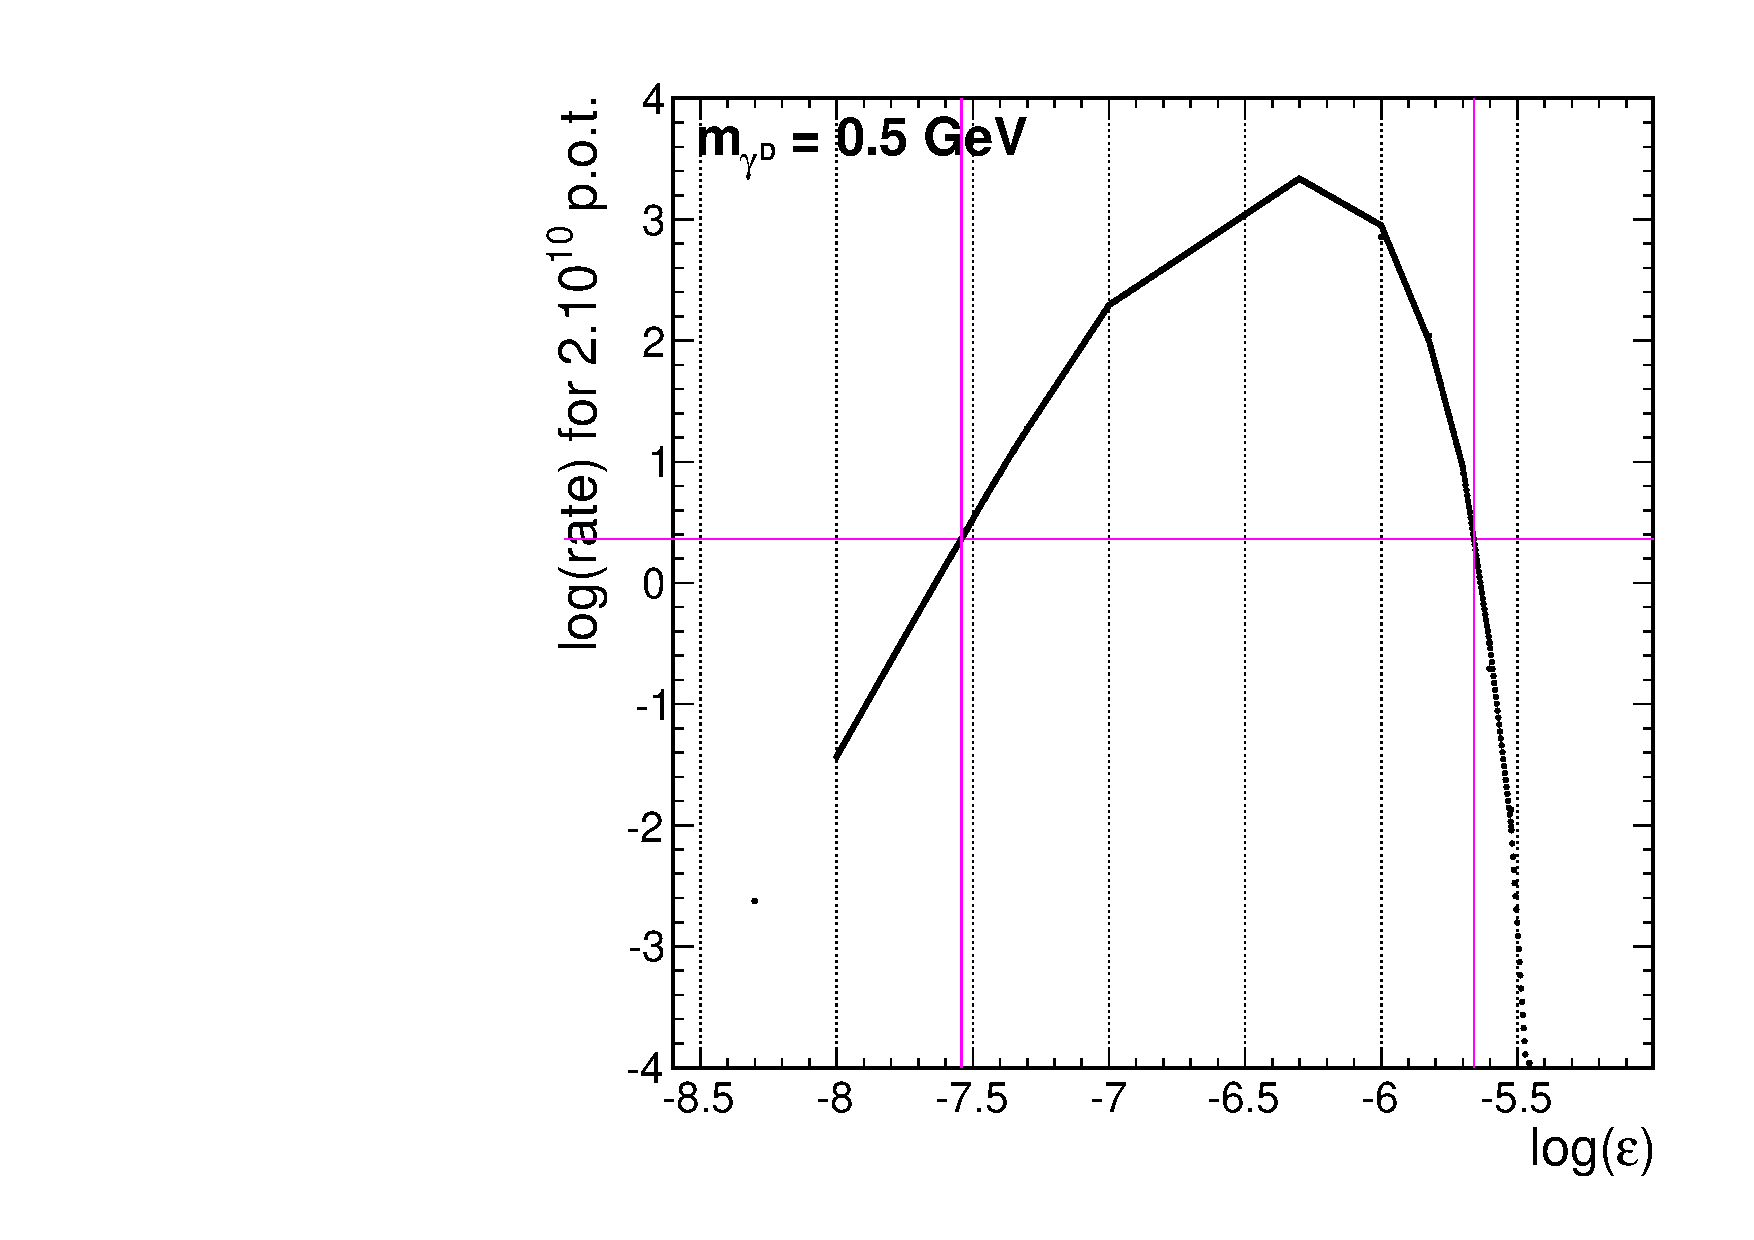
\includegraphics[width=0.32\textwidth]{figures/CheckRate_hTest_meson_M5.pdf}
  \hfill
  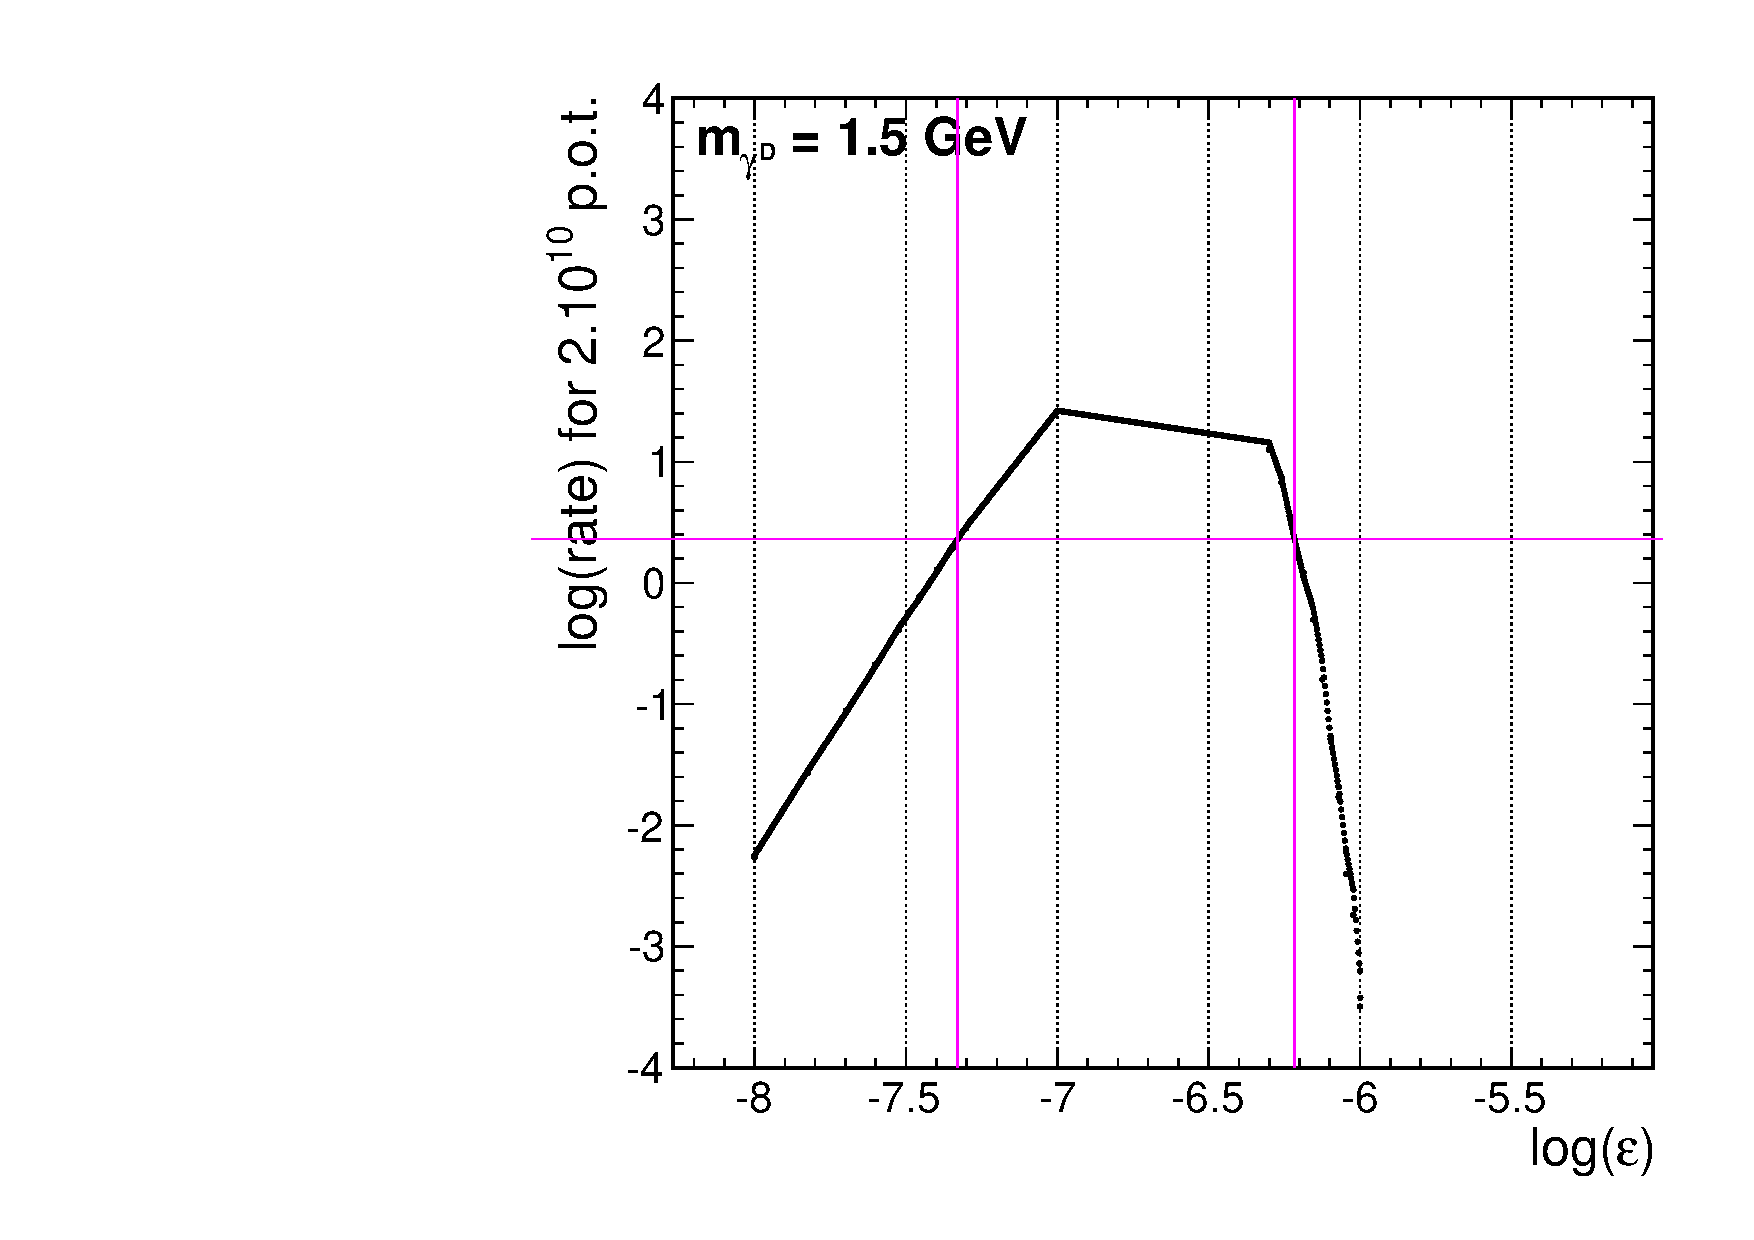
\includegraphics[width=0.32\textwidth]{figures/CheckRate_hTest_pbrem_M15.pdf}
  \hfill
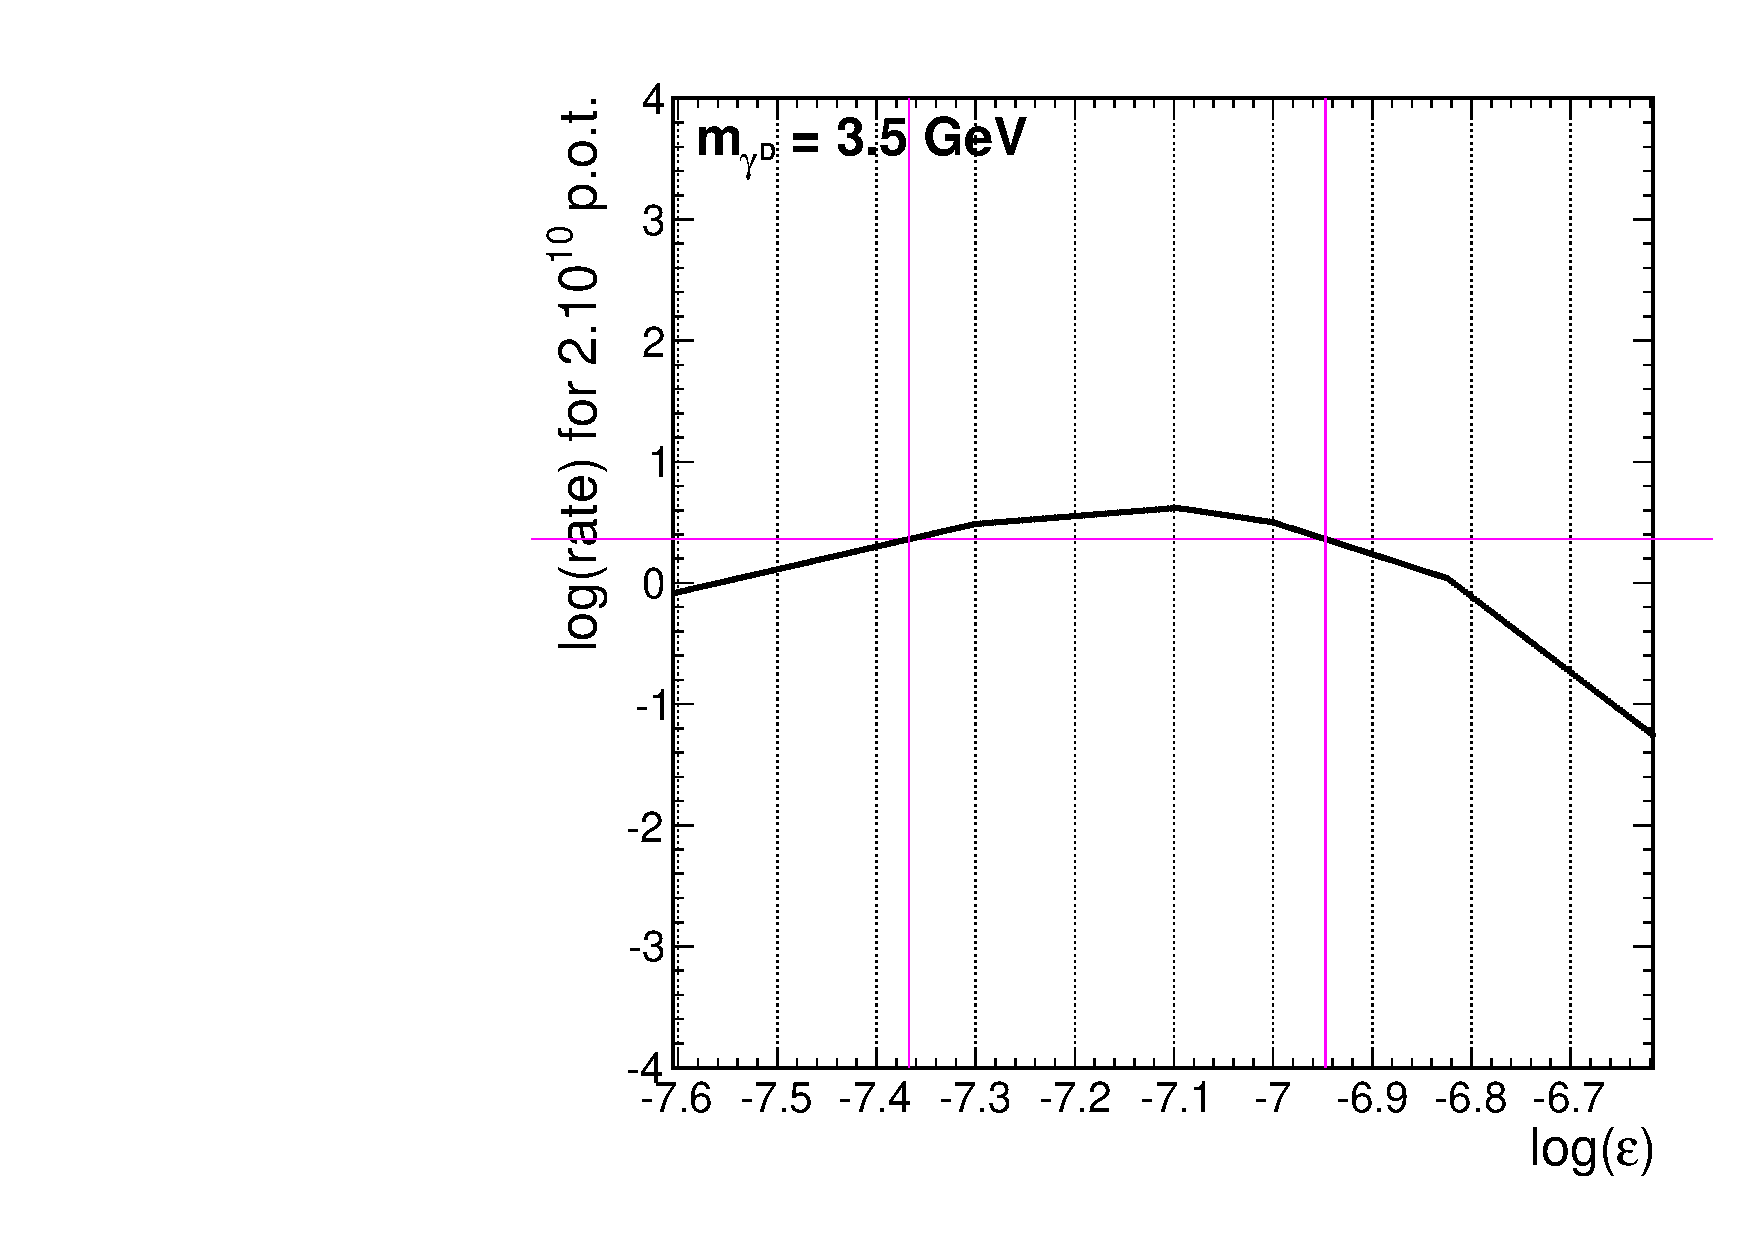
\includegraphics[width=0.32\textwidth]{figures/CheckRate_hTest_qcd_M35.pdf}\\
\caption{Expected rate as a function of $\varepsilon$, for \mDP$=0.5$ (left),
  1.5 (middle) or 3.5 (right) GeV and meson, proton bremsstrahlung or QCD production,
  respectively.}
\label{fig:ratevseps}
\end{figure}


The 90\% CL exclusion contour is shown in figure~\ref{fig:sensitivity}
for the three production mode studied, in the (\mDP,$\varepsilon$)
plane. Exclusion contours from theoretical constraints, existing and
other planned experiments sensitive to this process are overlayed. The
SHiP experiment is found to have a unique sensitivity in the mass
region m$_{\gamma^{\mathrm{D}}}$ ranging between XX and XX GeV, and
$\varepsilon$ ranging between XX and XX.

An alternative scenario in which the \DP would couple only to leptons
is also considered (``leptophilic'' case) and exclusion contour shown
in figure~\ref{fig:sensitivityLep}.

\begin{figure}[h!]
  \centering
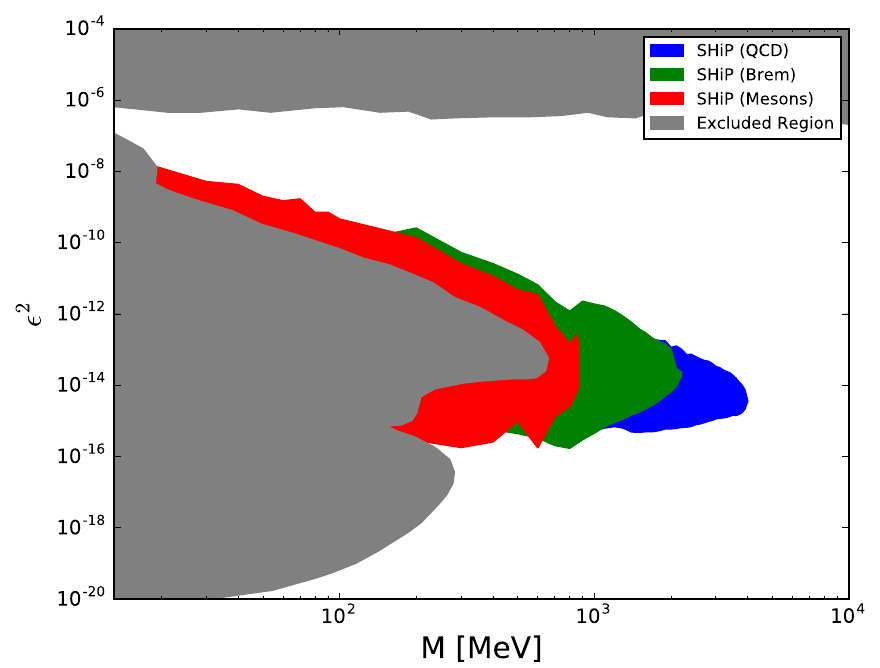
\includegraphics[width=1.\textwidth]{figures/sensitivity.png}
\caption{Expected 90\% exclusion region as a function of the dark
  photon mass and of the kinetic mixing parameter $\varepsilon$, for
  the three production modes studied.}
\label{fig:sensitivity}
\end{figure}

\begin{figure}[h!]
  \centering
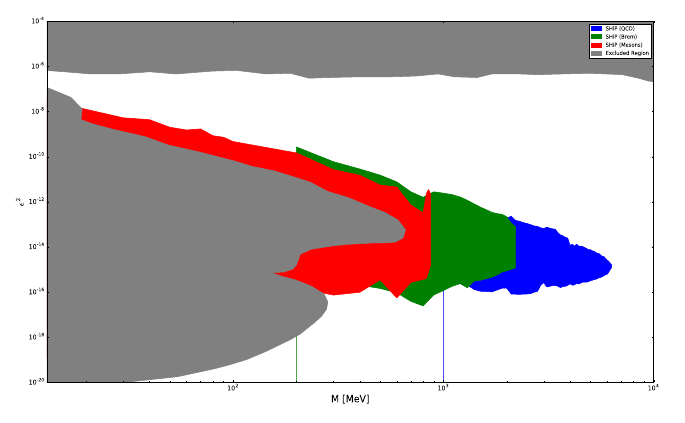
\includegraphics[width=1.\textwidth]{figures/sensitivityLeptophilic.png}
\caption{Expected 90\% exclusion region as a function of the dark
  photon mass and of the kinetic mixing parameter $\varepsilon$, for
  the three production modes studied, in scenarios where the \DP
  couples only to standard model leptons.}
\label{fig:sensitivityLep}
\end{figure}



\section{Conclusion}
\label{sec:concl}


The sensitivity of the SHiP detector has been investigated for the
simplest vector portal model, whereby the only hidden-sector particle
connecting to SM particles is a dark photon. The model is fully
parametrised by only two parameters, the mass of the dark photon \mDP
and the kinetic mixing parameter $\varepsilon$. Three different
production mechanisms have been investigated, namely the production
via meson decays from non-diffractive proton-proton interactions, by
proton bremsstrahlung and by QCD parton-parton interaction. Only the
primary proton-proton interaction is taken into account, secondaries
from hadronic interactions in cascade decays could lead to additional
sensitivity and will be the object of future work. The dark photon is
assumed to decay to pairs of fermions, and only decay channels
producing at least two charged particles coming from a common vertex
are used. With the selection applied, no background event is expected
and 90\% CL exclusion contours are extracted and compared with those
from theoretical constraints and other existing or planned
experiments. The SHiP detector is expected to have a unique
sensitivity for m$_{\gamma^{\mathrm{D}}}$ ranging between XX and XX
GeV, and $\varepsilon$ ranging between XX and XX.



% ****************************************************************************
% BIBLIOGRAPHY AREA
% ****************************************************************************
\cleardoublepage
\bibliographystyle{ieeetr}
\bibliography{dp_paper}

\end{document}
